\paragraph{From clean inputs to pure noise.}
\label{app:newinput-interpolation}
We measure how much of each atomic space survives when clean MNIST inputs are gradually replaced by uniform noise, following Appendix~\ref{app:methods-newinput}. Most hidden-layer directions survive throughout. Intermediate mixtures constrain the spaces more than pure noise, while the readout loses a larger and more seed-dependent fraction (Figure~\ref{fig:newinput-shift}). Thus moving farther from the training distribution need not remove more invariant directions.

\begin{figure}[!htbp]\centering
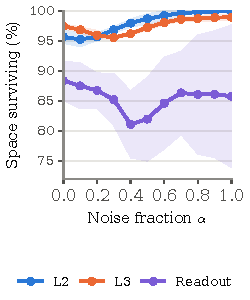
\includegraphics[width=1.499in]{newinput_interpolation.pdf}
\caption{Atomic-space survival under clean-to-noise interpolation, mean $\pm$ sample SD across three seeds. L3 has additional rank-cutoff sensitivity (Appendix~\ref{app:methods-newinput}), which preserves the qualitative trend.}
\label{fig:newinput-shift}
\end{figure}

\paragraph{SVHN inputs.}
Most of the hidden-layer spaces also survive SVHN images passed through the fixed MNIST preprocessing (Table~\ref{tab:newinput-svhn}). L2 survival is higher than for the clean MNIST reference in every seed; L3 and readout effects vary across seeds. Survival therefore depends on the additional feature and downstream constraints, rather than distribution shift alone.
\begin{table}[!htbp]\centering
\caption{Atomic-space survival (\%), mean $\pm$ sample SD across three seeds. SVHN uses the fixed MNIST representation. Rank sensitivity is assessed separately from seed variation.}
\label{tab:newinput-svhn}
\small\begin{tabular}{lccc}\toprule
Added inputs & L2 & L3 & Readout\\\midrule
Clean MNIST & $95.63 \pm 1.07$ & $97.39 \pm 0.42$ & $88.33 \pm 3.30$\\
SVHN & $98.41 \pm 0.91$ & $97.20 \pm 0.58$ & $87.30 \pm 3.04$\\\bottomrule\end{tabular}\end{table}

